\section{Análise de Requisitos}
\label{sec:analise-de-requisitos}

Dentre os dez requisitos do projeto, alguns exigem soluções envolvendo diversos sensores e técnicas específicas para seu cumprimento. Esta seção visa esclarecer a estratégia a ser adotada para algumas das funcionalidades necessárias do veículo.


\subsection{Matriz QFD}
\label{subsec:matriz-qfd}

\begin{table}[h]
	\centering
	\caption{Matriz QFD}
	\label{tab:qfd-brov}
	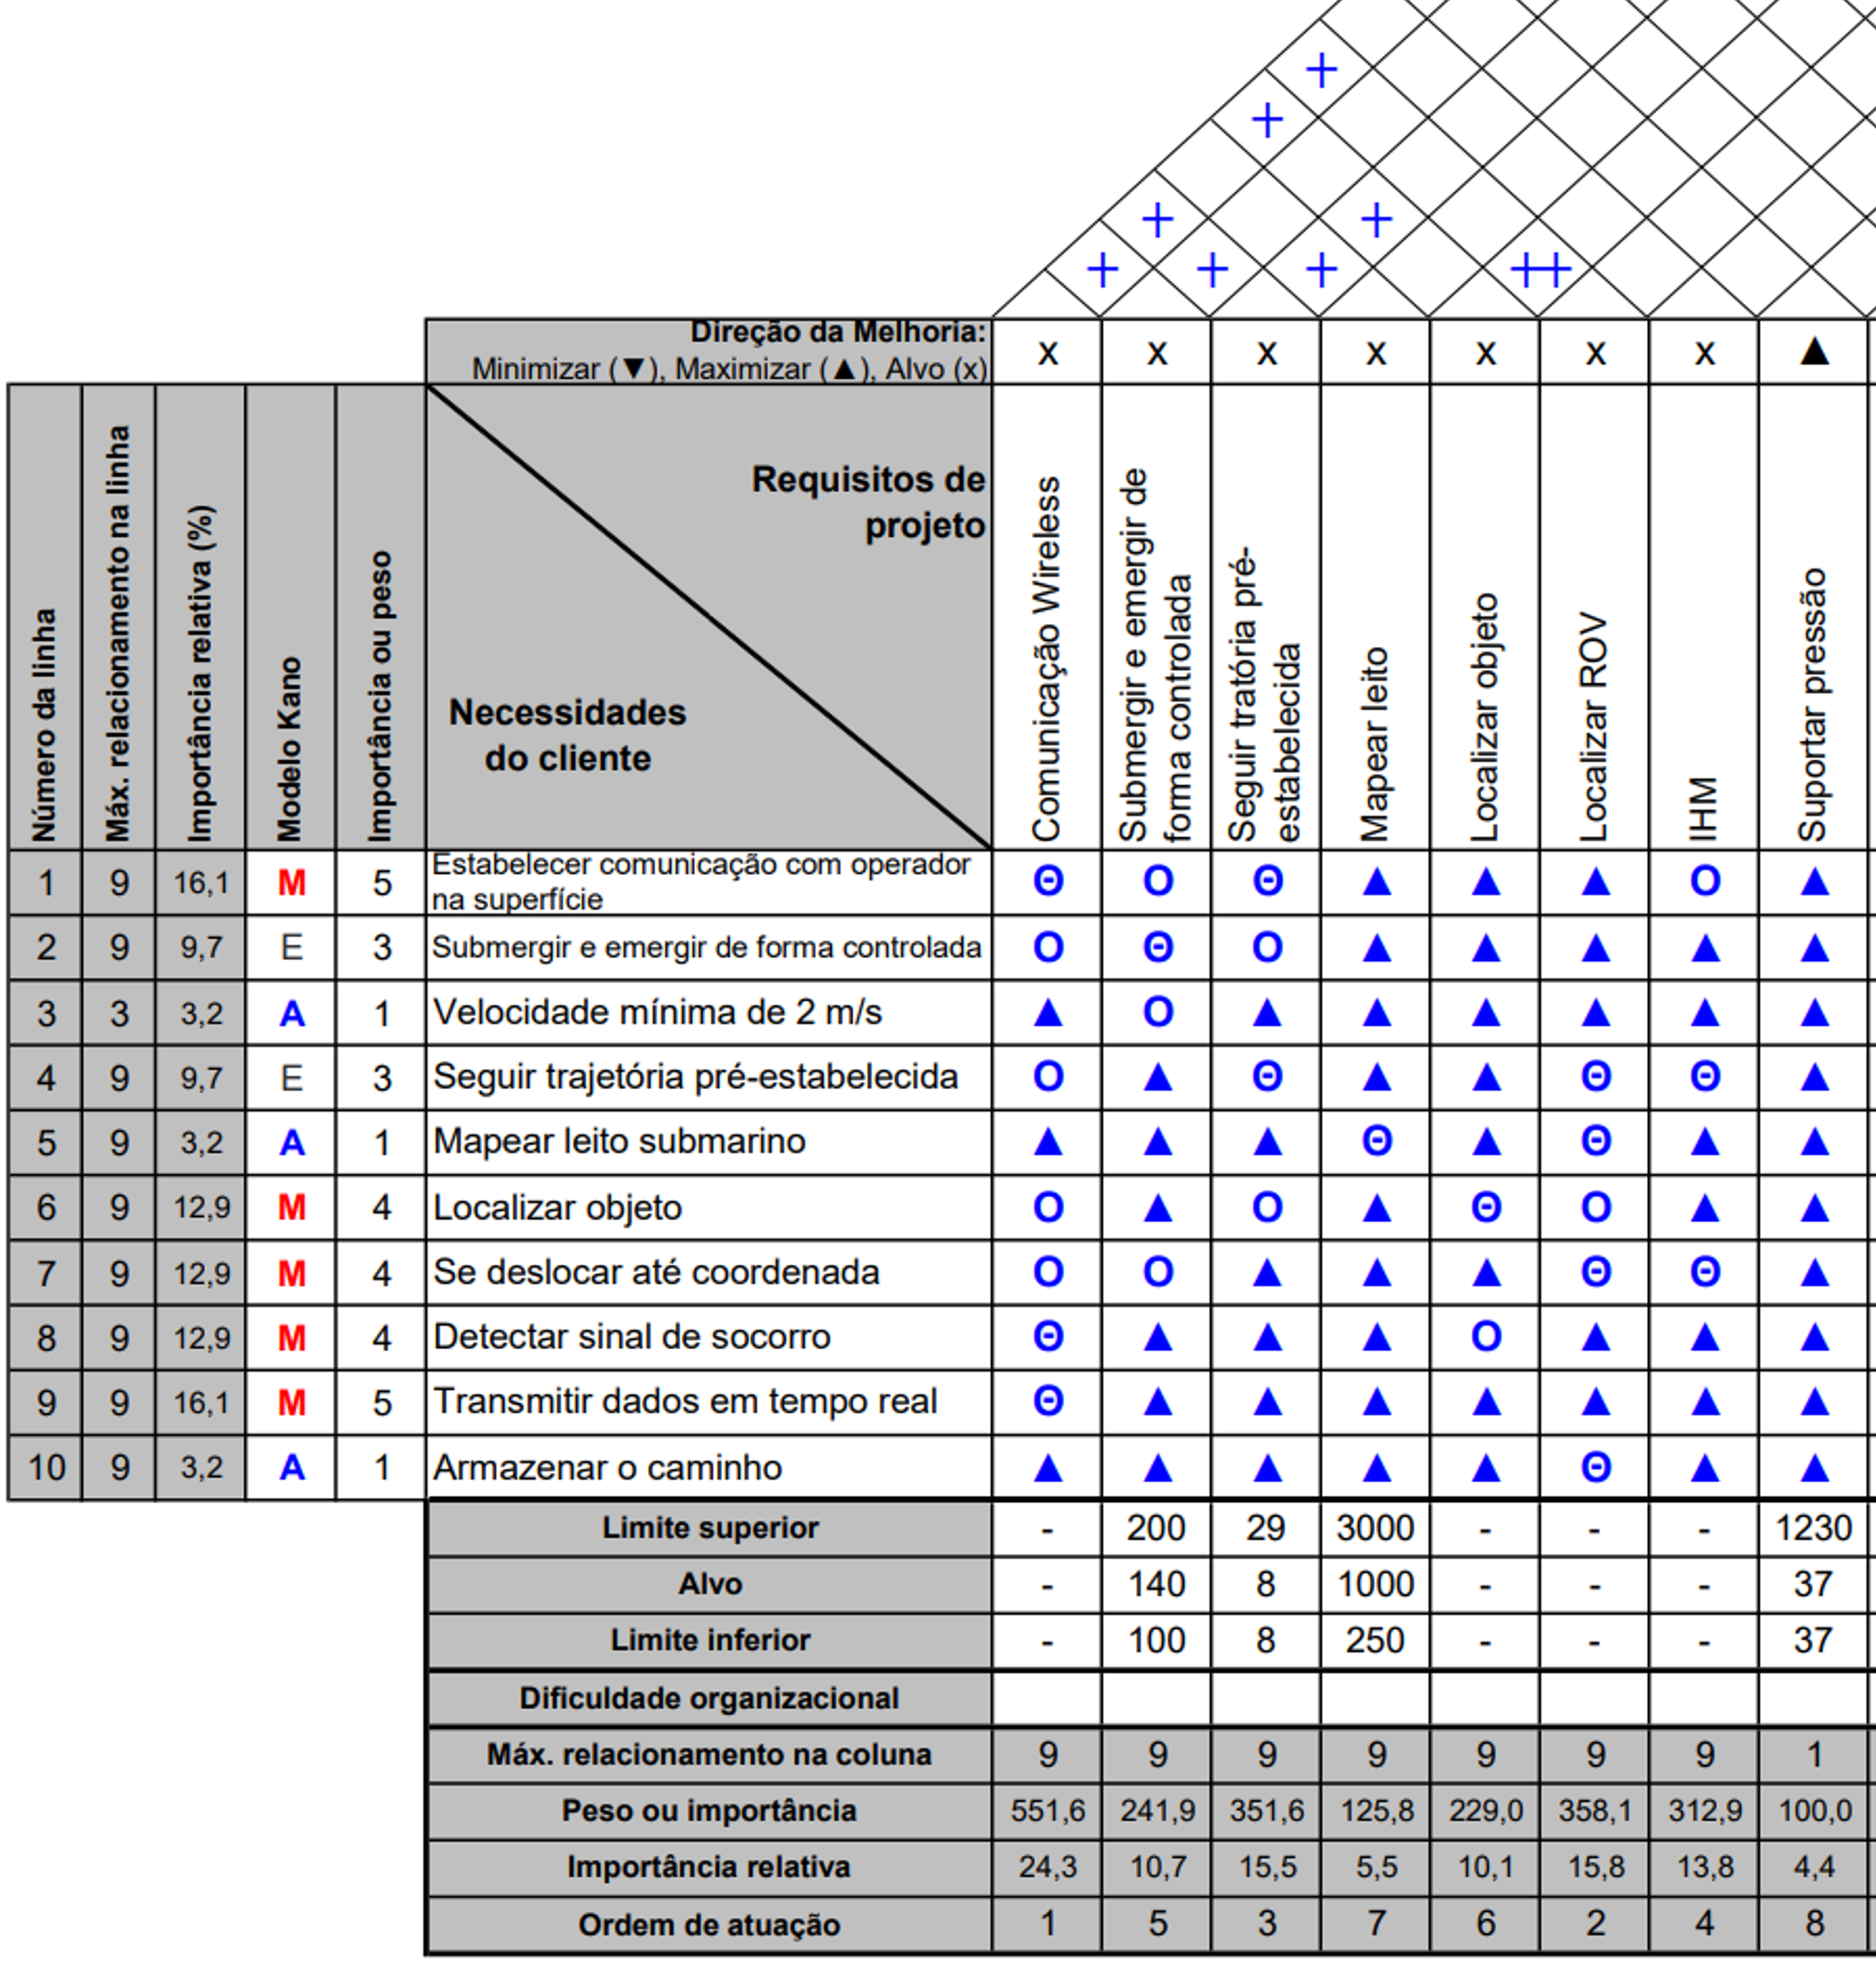
\includegraphics[width=1\linewidth]{images/QFD-BROV.png}\\
	\footnotesize Fonte: Autores
\end{table}

\subsection{Matriz Morfológica}
\label{subsec:matriz-morfologica}

\begin{table}[h]
	\centering
	\caption{Matriz morfológica}
	\label{tab:matriz-morfologica}
	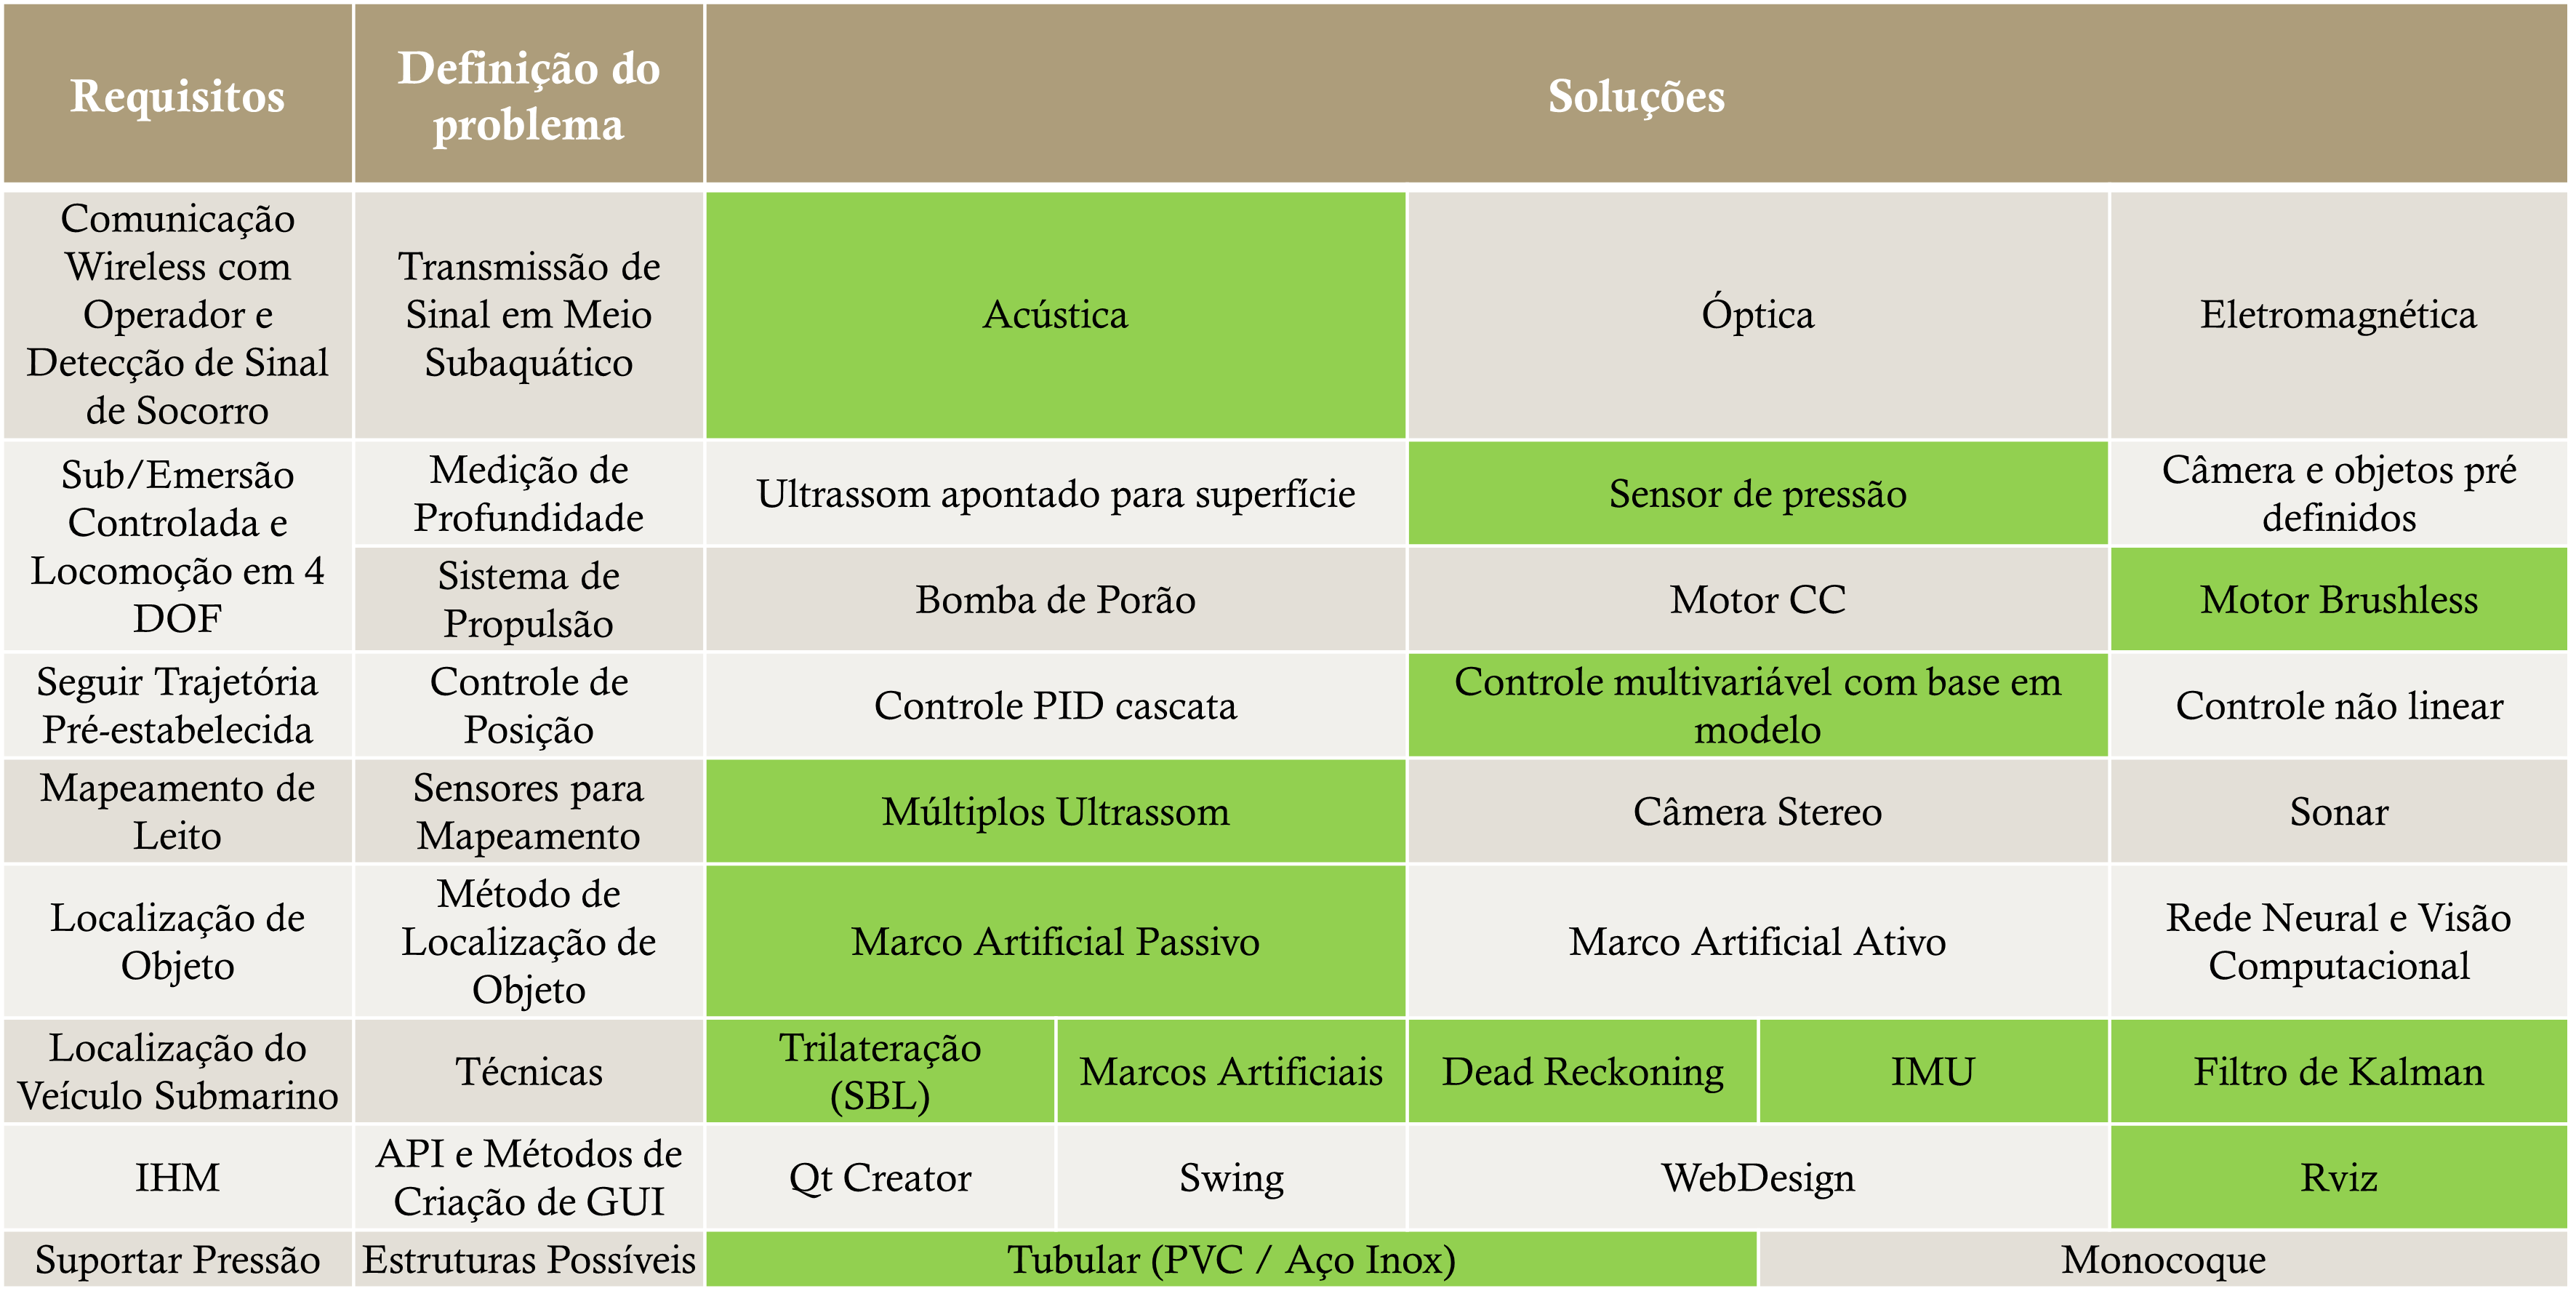
\includegraphics[width=1\linewidth]{images/Matriz-morfologica}\\
	\footnotesize Fonte: Autores
\end{table}

\subsubsection*{Localização}
\label{subsec:localizacao}

Um dos requisitos do projeto é a capacidade do veículo de se localizar no ambiente. Esse requisito tem impacto em diversos outros, pois não havendo sua localização, não se pode criar um mapa ou gerar uma trajetória a ser seguida. A localização do veículo consiste em saber a pose, os seis DOF (\textit{Degrees of Freedom}), do veículo em relação ao ambiente no qual está inserido. Dessa forma, deve-se ter inseridos no ambiente objetos conhecidos em poses conhecidas, os quais o veículo possa utilizar as detecções desses objetos para aferir sua pose no ambiente. Serão utilizados um sistema SBL (\textit{Short BaseLine}) e arucos como esses objetos conhecidos.

O sistema SBL é um conjunto de quatro \textit{beacons} acústicos que devem ficar emitindo um sinal acústico para o veículo, que atrávez da trilateração, é capaz de estimar a posição em XY desse sistema. Esse sistema em conjunto com o sensor de pressão e a inferência da posição em Z provê a todo momento a posição em XYZ do veículo. Dessa forma, somente falta a rotação em XYZ, que pode ser aferida a partir do giroscópio presente na IMU.

Mesmo já sendo possível obter a pose 6DOF do veículo com essas três soluções, a detecção de Arucos, \textit{dead-reckoning} e dados do acelerômetros também serão usados visando obtenção de uma localização mais precisa. A detecção por visão computacional de um aruco fixado ao ambiente possibilita a estimação da pose 6DOF do veículo, porém esse dado só está disponível enquanto o veículo aponta sua câmera para o aruco. O \textit{dead-reckoning} consiste em utilizar o modelo cinemático de deslocamento do veículo com a velocidade de cada propulsor para saber o deslocamento 6DOF que deve acontecer em um certo período, contudo, essa técnica pode agregar erros de modelagem, assim como de estimação do empuxo em cada propulsor. Por fim, o dado do acelerômetro integrado duas vezes provê dado de deslocamento de posição, mas como o erro do sensor também é integrado duas vezes, a técnica não é tão precisa. Dessa maneira, pelos problemas apresentados nesse parágrafo sobre a estimação de pose com acelerômetro, arucos e \textit{dead-reckoning}, essas serão usadas somente a partir da fusão por filtro de Kalman com as informações obtidas pelo SBL, sensor de pressão e giroscópio. O filtro de Kalman leva em consideração a precisão de cada dado durante sua fusão, então dados mais precisos tem mais peso do que dados imprecisos. 

Uma possibilidade são os próprios marcos artificiais, porém precisam estar em uma pose conhecida previamente, então com a estimativa de sua pose em relação ao veículo submarino, se calcula a pose do veículo no mundo. Outra possibilidade é a triangulação de sinal, com três emissores de pulsos acústicos ou ópticos com posições previamente conhecidas, consegue-se estimar a pose do veículo. Por fim, o \textit{dead-reckoning} também pode ser usado através de sensores inerciais e de estimadores de modelo cinemático e dinâmico do veículo. Esses componentes geram uma informação de deslocamento em relação a uma pose inicial, que é chamada de \textit{dead-reckoning}, ou odometria no caso de veículos terrestres.

\subsubsection*{Mapeamento}
\label{subsubsec:mapeamento}

O mapa será gerado a partir das medições de distância realizadas com os transdutores do fundo do veículo. Cada medição virará um voxel em um mapa de ocupação 3D.